%\documentclass[brudnopis,xodstep]{kdypl}%% opcja 'brudnopis' zwraca stopkę z nr wersji pracy i e-mailem, opcja 'xodstep' zwiększa odstęp do 1.3
% klasa posiada opcję 'licencjacka' dla prac licencjackich oraz 'magisterska' dla prac magisterskich
%\documentclass[magisterska]{kdypl}
\documentclass[licencjacka]{kdypl}
\usepackage[T1]{fontenc}
\usepackage{float}
\usepackage[utf8]{inputenc}
%\usepackage[latin2]{inputenc}
%\usepackage[cp1250]{inputenc}
\usepackage[MeX]{polski}
\usepackage{graphicx}
\usepackage{amsmath}
\usepackage{amsfonts}
\usepackage{amssymb}
\usepackage{color}
\usepackage[square,sort&compress]{natbib}
\providecommand{\BIBand}{i}
\usepackage[noload]{qtree}
\usepackage{indentfirst}

\renewcommand{\thesection}{\arabic{section}}


%\usepackage{makeidx}
%\makeindex

\newtheorem{df}{Definicja}
\newtheorem{tw}{Twierdzenie}
\newtheorem{lm}{Lemat}
\newtheorem{prz}{Przykład}

%Dedykacja (opcjonalna)
\dedicationpagetrue

\usepackage{hyperref}
\hypersetup{colorlinks,citecolor=black,filecolor=black,linkcolor=black,urlcolor=black}



% Opcjonalnie identyfikator dokumentu (drukowany tylko
% z włączoną opcją `brudnopis'):
\nrwersji {0.1}

%%%
% Przykładowe wykorzystanie pakietu fancyhdr do zdefiniowania
% tzw. żywej paginy (por. np. http://www.maths.soton.ac.uk/~ap/latex/fancyhdr.html)
%\usepackage{fancyhdr}
%\pagestyle{fancy}
%\fancyhf{}
%% 'Klasycznie', tj. wszystko w paginie górnej:
%\fancyhead[LE,RO]{\textbf{\thepage}}
%\fancyhead[LO]{\small\sffamily \nouppercase{\rightmark}}
%\fancyhead[RE]{\small\sffamily \nouppercase{\leftmark}}
%%
%\fancyfoot[LE,RO]{\textbf{\thepage}}
%\fancyhead[LE]{\small\sffamily \nouppercase{\leftmark}}
%\fancyhead[RO]{\small\sffamily \nouppercase{\rightmark}}
%%
%\renewcommand{\headrulewidth}{0.4pt}
%\renewcommand{\footrulewidth}{0.0pt}
%%

%
% Dane autora(ów):
\author{Katarzyna Masiarek}
\nralbumu{436421}
\email{katmas2@st.amu.edu.pl}

%Do oświadczenia:
\autor{}

% Tytuł pracy:
\title{Komunikacja człowiek - komputer\\HCI - dekodowanie informacji}%tytuł polski
\tytulang{}%tytuł angielski

%Do oświadczenia:
\tytul{}

% Kierunek:
\kierunek {Kognitywistyka}

% Rok obrony:
\date     {19/01/2019}

% Jeżeli nie podano miejsca zostanie wpisany `Poznań'
\miejsce {Poznań}

% Tytuł naukowy, imię i nazwisko promotora, np.:
%  dr Jan Kowalski
%  prof. dr hab.~Jan Kowalski
% itp.
\opiekun  {}


%
% Miejsce na deklaracje własnych poleceń:
\newcommand{\filename}[1]{\texttt{#1}}

% Cytowanie autor-rok
% \bibliographystyle{papalike}

\begin{document}

%%Polskie
%\begin{abstract}
%\noindent%Jeśli streszczenie składa się z jednego akapitu (a raczej powinno)
%abstrakt

%\end{abstract}

%\keywords{słowa kluczowe}

%%Angielskie
%\begin{abstracteng}
%\noindent%Jeśli streszczenie składa się z jednego akapitu (a raczej powinno)
%abstract

%\end{abstracteng}

%\keywordseng{keywords}

\maketitle

%%Odkomentowac ponizsze, jesli chcesz dedykowac swoja prace komus
%\dedication{Niniejszą pracę dedykuję\\...}
%\dedicationhere


\tableofcontents \thispagestyle{empty}




%\chapter*{Wstęp}\addcontentsline{toc}{chapter}{Wstęp}
%\introduction % przy zywej paginie
%Treść wstępu

%\chapter{Zadanie 1}\label{r1}

%A tu rozdział 1.
\newpage

\section{Informacje wstępne}
Do wykonania zadania użyto płytki OpenBCI Ganglion, której częstotliwość próbkowania wynosi $f_s = 200Hz$.

Nie mam informacji na temat osoby badanej.

\section{Wykonane zadanie}
Uzyskany podczas badania sygnał przefiltrowano przy użyciu następujących filtrów:
\begin{itemize}
	\item filtr pasmowo-zaporowy, którym wycięto częstotliwości $49Hz-51Hz$
	\item filtr dolnoprzepustowy z częstotliwością odcięcia $50Hz$
\end{itemize}

Na poniższej grafice przedstawione są rezultaty filtrowania.

\begin{figure}[H]
		\centering
		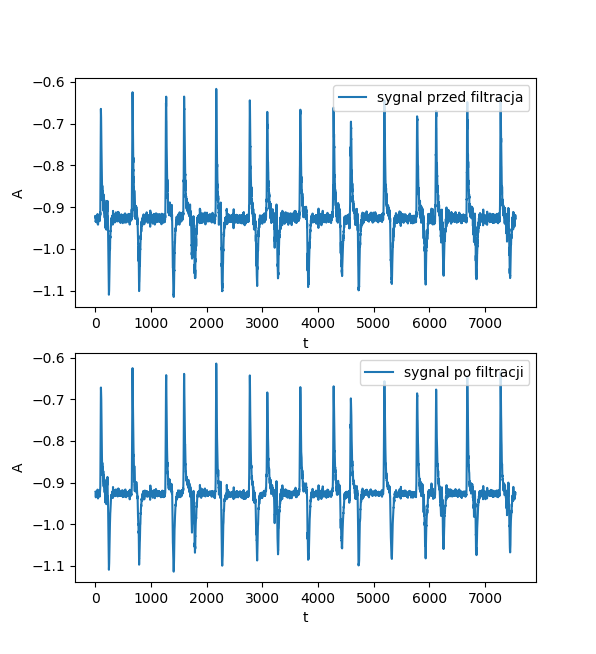
\includegraphics[scale=0.8]{sygnaly.PNG}
		\caption{Wykres sygnału przed i po filtracji}
		\end{figure}

\newpage		
Następnie przefiltrowany sygnał porównano z czasem wyświetlania kolejnych cyfr.
		
\begin{figure}[H]
		\centering
		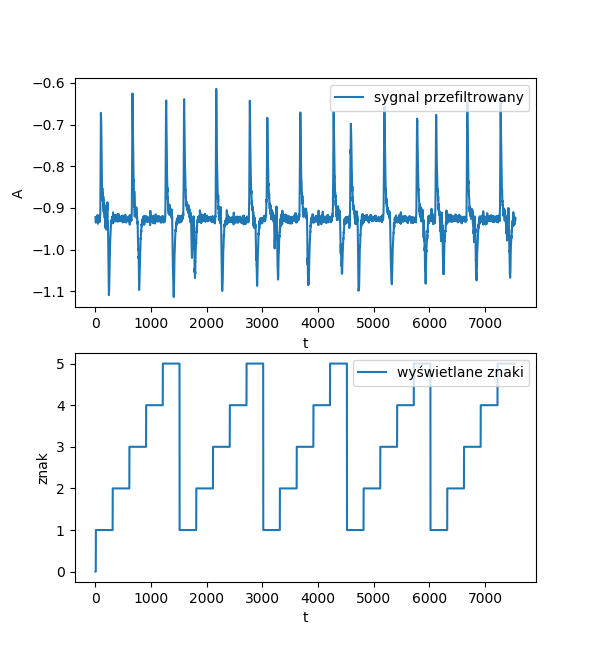
\includegraphics[scale=0.8]{sygCyf.PNG}
		\caption{Sygnał przefiltrowany i czasy wyświetlania kolejnych cyfr.}
		\end{figure}
		
Już z tego wykresu można odczytać, jakie cyfry wybrał badany, jednak zadanie to można ułatwić, wyświetlając oba sygnały na jednym wykresie, oraz przemnażając przefltrowany sygnał przez $-5$, tak, aby linie się nakładały.

Wykres taki oczywiście nie ma zadnej wartości poza ułatwieniem odczytania wybranych cyfr.

\begin{figure}[H]
		\centering
		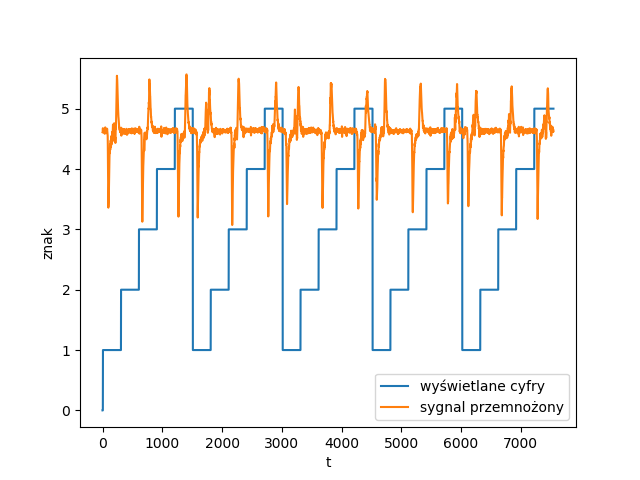
\includegraphics[scale=0.8]{combo.PNG}
		\caption{Nałożone na siebie sygnały}
		\end{figure}
		
Cyfry wybrane przez badanego to: 1, 3, 5, 1, 3, 5, 1, 3, 5,1, 3, 5.

Ponieważ nie byłam obecna podczas badania, nie mogę stwierdzić, czy kod taki był wybrany w rzeczywistości.

Link do programu: \url{}. 


%\chapter*{Zakończenie}
%\addcontentsline{toc}{chapter}{Zakończenie}







%
% Literatura:

%
% Spis tabel (jeżeli jest potrzebny):
%\listoftables
%
% Spis rysunków (jeżeli jest potrzebny):
%\listoffigures

%
% Skorowidz (opcjonalnie)
%\printindex



\end{document}

%\begin{figure}[H]
%		\centering
%		\includegraphics[scale=0.4]{pidB_oba.PNG}
%		\caption{Błąd pochodzący z modelu B. Oś 0Y wyskalowana jest w $10^{1}$}
%		\end{figure}